\documentclass{beamer}
\usetheme{Madrid}
\usepackage{amsmath}
\usepackage{ragged2e}
\graphicspath{ {./images/} }

\newcommand\myheading[1]{%
  \par\bigskip
  {\Large\bfseries#1}\par\smallskip}

\title{Introduction to Word2Vec}
\author{by Talentsprint Pvt. Ltd.}
\centering
\date{September 2020}

\begin{document}
\maketitle
\begin{frame}{Content}
	\begin{itemize}
		\item Introduction
		\item Types of Word2Vec
		\item How does Word2Vec produce word embeddings?
		\item Advantages and Disadvantages of CBOW
		\item Advantages and Disadvantages of Skip-grams
	\end{itemize}
\end{frame}

\begin{frame}{Introduction}
\begin{flushleft}
\begin{itemize}
	\item Word2Vec is a shallow, two-layer neural networks which is trained to reconstruct linguistic contexts of words.
	\item It takes as its input a large corpus of words and produces a vector space, typically of several hundred dimensions, with each unique word in the corpus being assigned a corresponding vector in the space.
	\item Word vectors are positioned in the vector space such that words that share common contexts in the corpus are located in close proximity to one another in the space.
	\item Word2Vec is a particularly computationally-efficient predictive model for learning word embeddings from raw text.
	\item It comes in two flavors, the Continuous Bag-of-Words (CBOW) model and the Skip-Gram model.
\end{itemize}
\end{flushleft}
\end{frame}

\begin{frame}{Contd ...}
	\begin{flushleft}
		Algorithmically these models are similar.\\
		\vspace{5pt}
		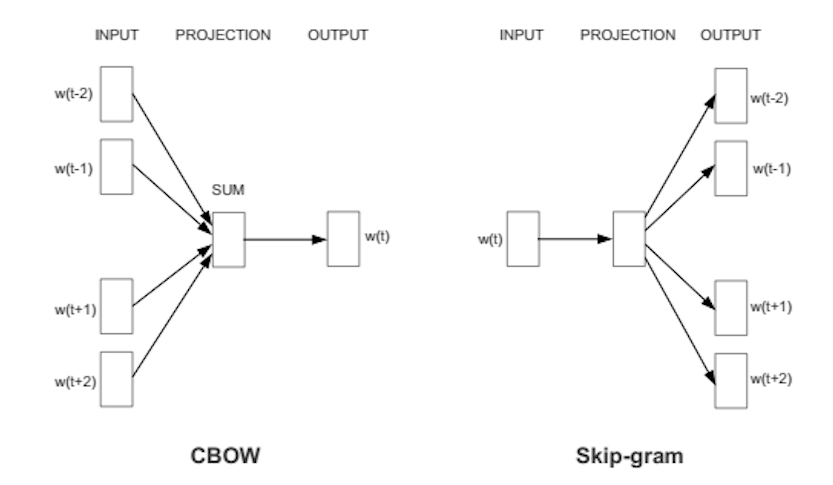
\includegraphics[height=7cm, width=11cm]{CBOW_skipgram}\\
	\end{flushleft}
\end{frame}

\begin{frame}{Types of Word2Vec}
\begin{flushleft}
\myheading{Continuous of Bag of Words:}
CBOW predicts target words (e.g. ‘mat’) from the surrounding context words (‘the cat sits on the’).\\
\vspace{10pt}
Statistically, it has the effect that CBOW smoothes over a lot of the distributional information (by treating an entire context as one observation). For the most part, this turns out to be a useful thing for smaller datasets.\\

\myheading{Skip-gram:}
Skip-gram predicts surrounding context words from the target words (inverse of CBOW).\\
\vspace{10pt}
Statistically, skip-gram treats each context-target pair as a new observation, and this tends to do better when we have larger datasets.
\end{flushleft}
\end{frame}

\begin{frame}{How does Word2Vec produce word embeddings?}
\begin{flushleft}
		Word2Vec is a simple neural network with a single hidden layer, and like all neural networks, it has weights, and during training, its goal is to adjust those weights to reduce a loss function. However, Word2Vec is not going to be used for the task it was trained on, instead, we will just take its hidden weights, use them as our word embeddings, and toss the rest of the model.
\myheading{Architecture:}
Take a large input vector, compress it down to a smaller dense vector and then instead of decompressing it back to the original input vector to output probabilities of target words.\\
\vspace{10pt}
Feeding a word as string into a neural network is not possible.
Instead, words are feeded as one-hot vectors, which is basically a vector of the same length as the vocabulary, filled with zeros except at the index that represents the word we want to represent, which is assigned “1”.\\

\end{flushleft}
\end{frame}

\begin{frame}{Contd...}
\begin{flushleft}
		The hidden layer is a standard fully-connected (Dense) layer whose weights are the word embeddings.\\
		\vspace{10pt}
The output layer outputs probabilities for the target words from the vocabulary.\\
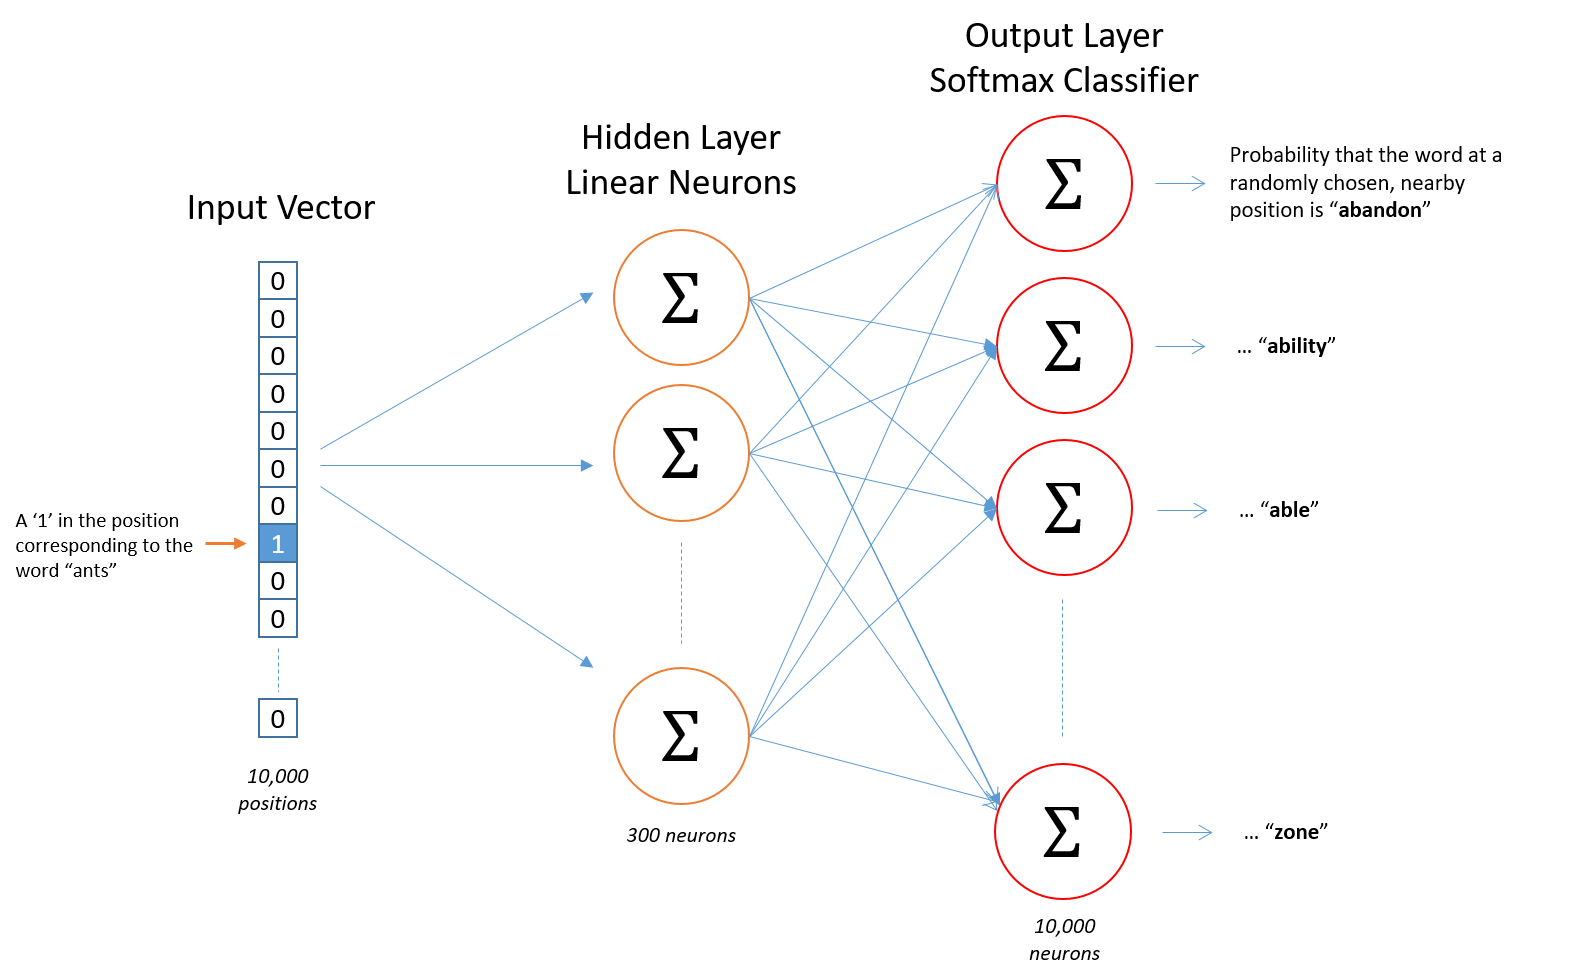
\includegraphics[height=5.7cm, width=12cm]{skip_gram_net_arch}
\end{flushleft}
\end{frame}

\begin{frame}{Contd...}
\begin{flushleft}
\begin{itemize}
	\item The input to this network is a one-hot vector representing the input word, and the label is also a one-hot vector representing the target word, however, the network’s output is a probability distribution of target words, not necessarily a one-hot vector like the labels.
	\item The rows of the hidden layer weight matrix, are actually the word vectors (word embeddings).
\end{itemize}
\myheading{CBOW:}
It tends to predict the probability of a word given a context. A context may be a single word or a group of words. For simplicity, Take a single context word and try to predict a single target word.\\
\vspace{5pt}
Suppose, we have a corpus \textbf{C = “Hey, this is sample corpus using only one context word.”} and we have defined a context window of 1. This corpus may be converted into a training set for a CBOW model as follow. The input is shown below. The matrix on the right in the below image contains the one-hot encoded from of the input on the left.
	\end{flushleft}
\end{frame}
\begin{frame}{Contd...}
\begin{flushleft}
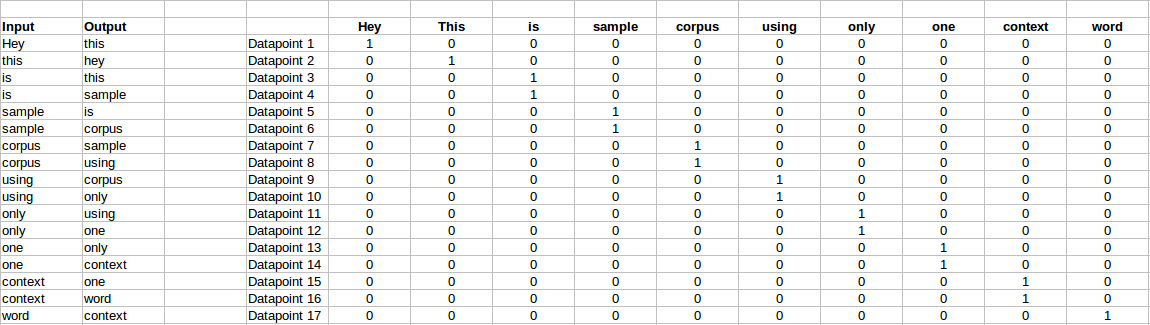
\includegraphics[height=6cm, width=12cm]{cbow1}
	 The target for a single datapoint say Datapoint 5 is shown as below\\
"Hey	this	is	sample	corpus	using	only	one	context	word"\\
0	0	0	1	0	0	0	0	0	0
	\end{flushleft}
\end{frame}

\begin{frame}{Contd...}
\begin{flushleft}
This matrix shown in the above image is sent into a shallow neural network with three layers: an input layer, a hidden layer and an output layer. The output layer is a softmax layer which is used to sum the probabilities obtained in the output layer to 1. Now let us see how the forward propagation will work to calculate the hidden layer activation.\\
\vspace{10pt}
The flow is as follows:
\begin{itemize}
	\item The input layer and the target, both are one- hot encoded of size [1 X V]. Here V=10 in the above example.
	\item There are two sets of weights. one is between the input and the hidden layer and second between hidden and output layer.
Input-Hidden layer matrix size =[V X N] , hidden-Output layer matrix  size =[N X V] : Where N is the number of dimensions we choose to represent our word in. It is arbitary and a hyper-parameter for a Neural Network. Also, N is the number of neurons in the hidden layer. Here, N=4.
\end{itemize}
	\end{flushleft}
\end{frame}

\begin{frame}{Contd...}
\begin{flushleft}
\begin{itemize}
	\item There is a no activation function between any layers.( More specifically, I am referring to linear activation)
	\item The input is multiplied by the input-hidden weights and called hidden activation. It is simply the corresponding row in the input-hidden matrix copied.
	\item The hidden input gets multiplied by hidden- output weights and output is calculated.
	\item Error between output and target is calculated and propagated back to re-adjust the weights.
	\item The weight  between the hidden layer and the output layer is taken as the word vector representation of the word.
\end{itemize}
	\end{flushleft}
\end{frame}
\begin{frame}{Contd...}
\begin{flushleft}
We saw the above steps for a single context word. Now, what about if we have multiple context words? The image below describes the architecture for multiple context words.

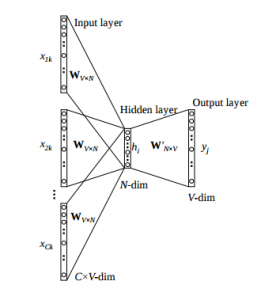
\includegraphics[scale=0.6]{cbow2}
\end{flushleft}
\end{frame}
\begin{frame}{Contd...}
	\begin{flushleft}
		The image above takes 3 context words and predicts the probability of a target word. The input can be assumed as taking three one-hot encoded vectors in the input layer as shown above in red, blue and green.\\
\vspace{10pt}
So, the input layer will have 3 [1 X V] Vectors in the input as shown above and 1 [1 X V] in the output layer. Rest of the architecture is same as for a 1-context CBOW.\\
\vspace{10pt}
The steps remain the same, only the calculation of hidden activation changes. Instead of just copying the corresponding rows of the input-hidden weight matrix to the hidden layer, an average is taken over all the corresponding rows of the matrix. We can understand this with the above figure. The average vector calculated becomes the hidden activation. So, if we have three context words for a single target word, we will have three initial hidden activations which are then averaged element-wise to obtain the final activation.
	\end{flushleft}
\end{frame}
\begin{frame}{Contd...}
	\begin{flushleft}
	\myheading{Skip-Gram Model}
	Input layer  size – [1 X V], Input hidden weight matrix size – [V X N], Number of neurons in hidden layer – N, Hidden-Output weight matrix size – [N X V], Output layer size – C [1 X V]\\
\vspace{10pt}
In the above example, C is the number of context words=2, V= 10, N=4
		\begin{itemize}
			\item The hidden activation corresponding to the input one-hot encoded vector. It is basically the corresponding row of input-hidden matrix copied. (R)
			\item The weight between the hidden layer and the output layer is calculated. (Y)
			\item The matrix multiplication of hidden activation and the hidden output weights is calculated. (B)
			\item Each row of the B matrix is converted into its softmax probabilities individually (G).
		\end{itemize}
	\end{flushleft}
\end{frame}

\begin{frame}{Contd...}
	\begin{flushleft}
\begin{itemize}
	\item The one hot encoded vectors of the two context words(target) is calculated. (T)
			\item Error is calculated by substracting the first row of the T from the first row of the G(output) element-wise. This is repeated for the next row. Therefore, for n target context words, we will have n error vectors.
			\item Element-wise sum is taken over all the error vectors to obtain a final error vector.
			\item This error vector is propagated back to update the weights.
			\end{itemize}
\end{flushleft}
\end{frame}
\begin{frame}{Advantages and Disadvantages of CBOW}
	\begin{flushleft}
\myheading{Advantages:}
	\begin{itemize}
	\item Being probabilistic is nature, it is supposed to perform superior to deterministic methods(generally).
	\item It is low on memory. It does not need to have huge RAM requirements like that of co-occurrence matrix where it needs to store three huge matrices.
	\end{itemize}
\myheading{Disadvantages:}
	\begin{itemize}
	\item CBOW takes the average of the context of a word (as seen above in calculation of hidden activation). For example, Apple can be both a fruit and a company but CBOW takes an average of both the contexts and places it in between a cluster for fruits and companies.
	\item Training a CBOW from scratch can take forever if not properly optimized.
	\end{itemize}
\end{flushleft}
\end{frame}
\begin{frame}{Advantages and Disadvantages of Skip-grams}
	\begin{flushleft}
\myheading{Advantages:}
	\begin{itemize}
	\item Skip-gram model can capture two semantics for a single word. i.e it will have two vector representations of Apple. One for the company and other for the fruit.
	\item Skip-gram with negative sub-sampling outperforms every other method generally.
	\end{itemize}
\myheading{Disadvantages:}
	\begin{itemize}
	\item Skip-gram model fails to identify the combined word phrases like "New York".
	\item Training a Skip-gram from scratch can take forever if not properly optimized and requires lot of RAM memory.
	\end{itemize}
\end{flushleft}
\end{frame}
\begin{frame}
\huge{\centerline{The End}}
\end{frame}
\end{document}